\documentclass[%
% if you want to use pdflatex, uncomment the following line
%pdftex
% if you have difficulties with fonts uncomment the following line
%notimes
]{algotel}
\usepackage[latin1]{inputenc}
\usepackage{draftwatermark}
\SetWatermarkText{DRAFT}
\SetWatermarkScale{1}
\usepackage{ mathrsfs }
\usepackage{mathtools}  
\usepackage{amsmath}
\usepackage{graphicx} % omit 'demo' for real document
\usepackage{relsize}
\usepackage{lmodern}
\usepackage{slantsc}
\usepackage{amssymb}
\usepackage{tabulary}
\usepackage{subcaption}
\usepackage{booktabs}

\usepackage[boxed,vlined]{algorithm2e}
\SetKwRepeat{Do}{do}{while}
\usepackage[toc,page]{appendix}
\usepackage{multicol}
\usepackage{blindtext}
\usepackage[francais]{babel}
\usepackage{algorithmic}


\newcommand{\exedout}{%
  \rule{0.8\textwidth}{0.5\textwidth}%
}

\author{Nicolas Herbaut\addressmark{1}\addressmark{2}\thanks{The work performed for this paper has been partially funded by the FP7 IP T-NOVA European Project (Grant Agreement 619520) and the FUI French National Project DVD2C}{\ }
  \and Daniel N�gru\addressmark{1}}


\title[]{D�ploiement d'un chaine de service de livraison de contenu multimedia sur une infrastructure d'op�rateur bas�e sur SDN-NFV}

\address{\addressmark{1}Univ. Bordeaux, LaBRI, UMR 5800, F-33400 Talence, France
\addressmark{2}Viotech Communications, Versaille, France

}


\keywords{SDN, NFV, Service Chaining, Content Delivery, CDN ISP Collaboration}

\begin{document}
\maketitle

\begin{abstract}
La consommation de videos "over the top" a chang� la donne pour les acteurs du monde de la livraison de contenu. La chaine de valeur a gliss� progressivement en faveur des fournisseurs de contenus et des r�seaux de livraison de contenu et au d�triment des fournisseurs d'acc�s.
Notre contribution propose un nouveau mod�le de collaboration entre ces diff�rents acteurs par la cr�ation d'une plateforme o� sont d�ploy�es des cha�nes de service de distribution de contenu. Nous �tudions en particuliers les solutions de placement de ces fonctions r�seaux sur un substrat de serveur virtualis�s au sein d'un r�seau respectant l'approche Software Defined Network (SDN) dans lequel sont d�ploy�es des infrastructures de virtualisation de fonction r�seau (NFV).
\end{abstract}

\section{Introduction}
Video streaming is the number one service on the current Internet. As the Internet was not originally designed for streaming high quality video, delivering this massive amount of content is a challenging task. 
One solution to mitigate those issues is to use Content Delivery Networks (CDN). 
CDNs have been created to improve network performance for end-users while at the same time limiting the need for Content Providers (CP) to own an infrastructure \cite{pathan2014cloud}.
By deploying servers in strategic locations, CDN Providers assign users to a close-by server, thus reducing hop count and avoiding congestion occurrences.

In this very competitive market, the majority of Internet Service Providers (ISP) are being kicked out of the video delivery value chain and is struggling to minimize the drop in their revenues \cite{wulf_carrier_2010}.  
However, even if their business role in the delivery part is challenged by CDNs, ISPs still hold a valuable asset: they can manage the whole network, i.e., the complete routing process end-to-end. 

The envisioned solution is a collaboration model for ISP and CDN around a Network Function Virtualization (NFV) architecture.
We propose a solution where ISPs can manage a NFV infrastructure where CDNs can run their caching software as NFVs through a virtual CDN (vCDN) network function.
It is a win-win approach since CDNs can expand their coverage dynamically without buying new servers and ISPs can increase their revenue by billing them while reducing inter-AS traffic.

The rest of the paper is organized as follows.
Section~\ref{sec:architecture} describes the architecture of the solution. Section~\ref{sec:results} presents the results of the model. We conclude the paper an present future work in Section~\ref{sec:conclusion}\footnote{the mathematical models \& algorithms are presented in the extended on line version of this paper: http://www.labri.fr/perso/nherbaut/algotel2016}.

\section{A NFV/SDN platform for virtual CDN deployment in the ISP's network\label{sec:architecture}}

CDN and ISP do not naturally collaborate.
They have their own specific problems to solve resulting in conflicting outcomes \cite{jiang_cooperative_2009}.
In order to overcome this collaboration challenges, we propose a solution matching ISP's connectivity "supply" with the CDN's connectivity "demand".




\begin{figure}
\centering
\begin{minipage}{0.45\textwidth}
\centering
	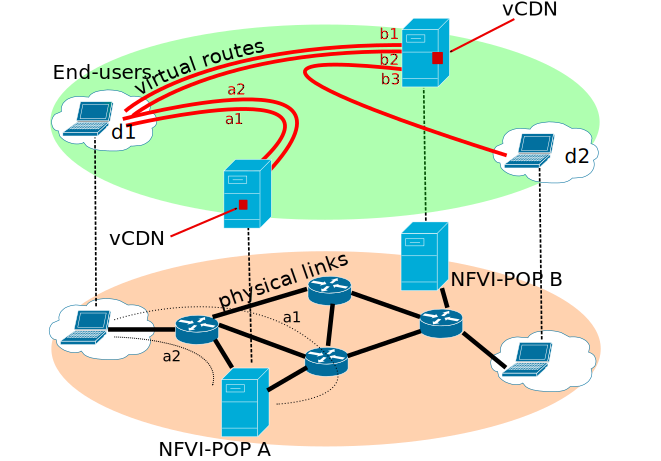
\includegraphics[width=1\textwidth]{fig/overlay.pdf}
	\caption{ vCDN deployed in ISP Network 
    \label{fig:overlay}}
\end{minipage}\hfill
\begin{minipage}{0.45\textwidth}
\centering
	\includegraphics[width=1\textwidth]{fig/results.pdf}
	\caption{ Impact of Service Chain transformation on the rate of successful embedding	
    \label{fig:results}} 
\end{minipage}

\end{figure}



\subsection{High-Level Architecture}

Our proposal, as depicted in Figure~\ref{fig:overlay}, aims at instantiating a Network Function Virtualization (NFV) platform within the ISP Network capable of hosting, among others, Virtual CDN (vCDN) services. 
The vCDNs hereby deployed keep being operated by the CDNs algorithms.

This platform is distributed amongst several NFV infrastructure points of presence (NFVI-POP), at the edge of the network. 
NFVI-POPs are data centers that provide compute resources (CPU, RAM, HDD) to run virtual Network Functions (vNF) on, following a "Network Function as a Service" (NFaaS) approach.

On top of the compute part, virtual routes are defined between end-users and vCDN instances. 
This solution masks the underlying network to the CDNs and keep the ISP topology and features secret, following a private "Connectivity as a Service" (CaaS) approach.

By combining and orchestrating both network and compute resources together, the ISPs can resell them to third parties.
Following this concept, ISPs are capable of contracting Service Level Agreement (SLA) with the CDNs for them to run their vCDN Network Functions.
For example, a CDN can contract with an ISP to organize the delivery of 5.000 concurrent HD streaming sessions in the Bayonne metropolitan area, with guaranteed Quality of Service.

\subsection{Implementing the Content Delivery Service}

While an SLA is a good way for CDNs to formulate their business needs, it does not specify technically how ISPs should perform the instantiation on their network.
In this section, we present the translation of the SLA into a Content Delivery Service Chain.

\subsubsection*{The canonical model}
The canonical representation of Content Delivery Service is depicted Figure~\ref{fig:canonical}, where two distinct flows emerge from the route note $s$ where End-Users get their connectivity from. 
On one hand, we have the $s\rightarrow CDN$ flow which represents the traditional path to content delivery: packets flow through the ISP autonomous system (AS) and reach the separate CDN AS.
On the other hand, the $s \rightarrow vCDN$ flow is targeted at an NFVI-POP within the ISP AS.
It is the enhanced distribution path on which the CDN want to apply the SLA. It has tighter network constraints (low delay, high bandwidth) and can hence deliver better quality videos.

\subsubsection*{Leveraging Virtual Home Gateways}
CDNs use DNS redirection technique to specify to which server content traffic need to be routed. This application-layer method works with the granularity of domain names.
ISPs can benefit from their full control of the network to switch to an SDN approach bringing more flexibility.

To deploy configuration to network devices, the SDN approach relies on "southbound technologies"  which can be limited in features.
For instance, Open flow is SDN's most used southbound protocol.
To this day, it can operate only on the levels 1 to 4 of the OSI layer model.
This limits the possibilities left by the CDNs to choose the right server, as all the requests sent to a particular domain are resolved by the same DNS request and sent to the same server regardless of the actual presence of the content on this server. Needing to retreive the content through the CP network would defeat the purpose of having an SLA as the performances would depend on another network.

To mitigate this issue, Virtual Home Gateways can be used to enhance content distribution \cite{etsi001}. 
vHG are virtual appliances that outsource traditional physical Home Gateway's Network Functions to the cloud, leaving a simple L2 bridge on the user premises. 
The vHG regroups several network functions, but in the present use case we focus on the routing function.
In a content delivery scenario, vHG can be seen as a transit network function able to flag outgoing flows according to L5-L7 rules, like HTTP URL matching.
vHG can therefore segregate traffic targeted toward vCDN from the one targeted to CDN.
This enable packets to follow distinct routes with distinct network characteristics.
For example, let's assume that a set of video files is cached in a vCDN. Each one is identified by its original URLs in the CP name space. 
Then, the CDN configures the mapping between original video URLs and their corresponding cached version. Finally, the vHG routes the requests made by the end-users the vCDN instance following a virtual route created at service mapping time, with guaranteed bandwidth and delay.
The remaining requests that don't match any URL are sent through a virtual route with no specific guarantees to the CDN AS.

\begin{figure}
\begin{subfigure}{0.31\textwidth}
\includegraphics[width=\linewidth]{fig/service.pdf}
	\caption{Canonical Representation}
	\label{fig:canonical}
\end{subfigure}
\hspace*{\fill} % separation between the subfigures
\begin{subfigure}{0.31\textwidth}
\includegraphics[width=\linewidth]{fig/service_chain.pdf}
	\caption{Implementation using vHG}
	\label{fig:vhg}
\hspace*{\fill} % separation between the subfigures
\end{subfigure}
\begin{subfigure}{0.31\textwidth}
\includegraphics[width=\linewidth]{fig/lb-service.pdf}
	\caption{With Load Balanced vHG}
	\label{fig:vhg-lb}
\end{subfigure}
\caption{Three representations of the same Service Chain} \label{fig:1}
\end{figure}



\subsubsection*{Service Chaining transformation}
\begin{figure}
	\center
	\includegraphics[width=.75\textwidth]{fig/service-mapping.pdf}
	\caption{ Service Chain Mapping
    \label{fig:service-mapping}}
\end{figure}
The resulting service can now be modeled as a Service Chain depicted in Figure~\ref{fig:vhg}.
The ISPs need to embed the Service Chain generated from the CDN SLA into their substrate network. 
This problem is known as Service Chain Embedding \cite{quinn2015problem} where we need to map a service graph $G^{S}=(N^{S},E^{S})$ to a substrate graph $G=(N,E)$ representing the real ISP network. Figure~\ref{fig:service-mapping} shows such a mapping. 

SLAs varies in the amount of physical resources needed and can be very demanding sometimes. In this context, it can be quite challenging for the ISPs to map a vNF to a single POP or to route the resulting traffic though a single route with enough bandwidth.
To ease this embeddings into the network, ISP can transform the canonical representation of the service into an other form by splitting vNFs and routes as shown Figure~\ref{fig:vhg-lb} known as path slitting. 
As nothing prevent vNFs to be allocated on the same POP, nor routes to be mapped to the same set of edges, the probability of  successful embeding for transformed model is at least equal to the canonical model.
Having traffic and resource split, however can ease service mapping on the substrate network, as each service and route need less resource for embeding.

\section{Results\label{sec:results}}
To evaluate our solution, we performed simulation on a real topology retrieved from an open database\footnote{http://www.topology-zoo.org/}.
We only considered transformations at the VHG level, by increasing the number of vHGs being load balanced and fairly spiting the traffic between them. Figure~\ref{fig:results} display the results of increasing the number of vHG while   picking traffic sources and sinks at random in the graph.
As we can see, splitting the path to vHG increases the probability of a successful embedding, up to a 10\% gain for 4 transformations wrt to the initial Service Chaining.

\section{\label{sec:conclusion}Conclusion and future work \label{sec:conclusion}}
We proposed a design for an ISP NFV collaboration platform in which CDNs can run their delivery functions. We modeled the problem of embedding a content delivery Service Chain over the ISP network, leveraging innovative network functions.

By just applying an algorithm that splits the traffic on several vNFs in the chain, we can see that it provides significant increase in the embedding acceptance ratio.
We plan to improve this algorithm by extracting topology information to help design a better transformation algorithm.
We are in the process of implementing a proof of concept of our approach in collaboration with an Operator, into which we will measure the performance in terms of peering traffic reduction,  quality of service for end-users and scalability. Furthermore, deriving an economic model of this new platform will permit us to analytically evaluate how the equilibrium/balance in revenue sharing is reached and a full win-win approach is achieved.



\nocite{}
\bibliographystyle{alpha}
\bibliography{algobib}
\pagebreak
\begin{appendices}
	\section{Service Mapping algorithm}
	\begin{algorithm}[H]
  \KwData{CDN's provided SLA}
  \KwResult{A Service Mapping $\mathscr{M}$ for SLA or rejection }
  
  $s \leftarrow $ canonical\_service(SLA)\;
  \Do{ true }{
		$\mathscr{M} \leftarrow solve(s)$\;
      \eIf{$\mathscr{M} = \emptyset $}{
      $s \leftarrow $ transform($s$)\;
      \If{$s = \emptyset$}{
      throw rejection\;
      }
      
      }{ return $\mathscr{M}$ \;}
    }
  \caption{Service Mapping algorithm}
\end{algorithm}

\section{Mathematical Model}

\subsection{Cost function}

We aim at maximize (\ref{eq1}) which incentive mapping to use the broader links for virtual routes. Note that the $\delta$ variable control for null bandwidth between nodes of the substrate network.

\begin{equation} \label{eq1}
			\sum_{
			\!\mathsmaller{
			(i,j)\in\mathscr{P}^{S}(s,x)
			}
			}{\quad\sum_{
			\!\mathsmaller{
			{(u,v)\in\mathscr{P}^{S}_{\mathscr{M}}(i,j)}
			}
			}{   \frac{b_{u,v}-(y^{i,j}_{u,v})}{\delta+b_{u,v}}         }}\\
\end{equation}
\subsection{Network function location unicity constraint}

Equation~(\ref{eq2}) assures that each network function is allocated only 1 node $u$ in the substrate.

\begin{equation}  \label{eq2}
		\sum_{u\in N} x_u^{i}=1, \forall i \in N^{S}
\end{equation}

\subsection{Substrate node constraint}

Equation~(\ref{eq3}) assures that each network function is allocated to a node that match the required capacity $c^{S}_{i}$.

\begin{equation} \label{eq3}
	\sum_{i \in N^{S} } x_{j}^{i} \times c_{i}^{S} \leq c_{u}, \forall u \in N		
\end{equation}

\subsection{Substrate edge capacity constraint}

Equation~(\ref{eq4}) assures that for each segment used to map service edge $(i,j)$ has enough bandwidth.

\begin{equation}\label{eq4}
	\sum_{(i,j)\in E^{S}}{y_{u,v}^{i,j}\times b_{i,j}^{S}} \leq b_{u,v}, \forall (u,v) \in E
\end{equation}


\subsection{Substrate edge delay constraint}

Equation~(\ref{eq5}) assures that each segment used to map service edge $(i,j)$ has a smaller delay that the one needed by the service.

\begin{equation}\label{eq5}
	y_{u,v}^{i,j}\times d_{u,v} \leq d_{i,j}^{S}, \forall (u,v) \in E, \forall (i,j) \in E^{S}
\end{equation}

\subsection{Flow conservation constraint}

Equation~(\ref{eq6}) implement classical flow conservation constraints.


\begin{equation}\label{eq6}
\sum_{v \in N}{y_{u,v}^{i,j}-y_{v,u}^{i,j}} = x_{u}^{i}-x_{u}^{j}, \forall (i,j) \in E^{S}, \forall u \in N / \{u \in  \mathscr{T}\}
\end{equation}

\subsection{Loop Constraints}
Equation~(\ref{eq7}) assures that there's no loop in the mapped service.
\begin{equation}\label{eq7}
y_{u,v}^{i,j}+y_{v,u}^{i,j} \leq 1, \forall (u,v) \in E, \forall (i,j) \in E^{S}
\end{equation}


\subsection{Domain Constraints}
Equations~(\ref{eq8})~and~(\ref{eq9}) represents domain constraints.
\begin{equation}\label{eq8}
x_{i}^{u}\in\{0,1\}
\end{equation}
\begin{equation}\label{eq9}
y_{u,v}^{i,j}\in\{0,1\}
\end{equation}


\section{Mathematical Notations}
  
\begin{table}[htbp]\caption{Notations}
\begin{center}% used the environment to augment the vertical space
% between the caption and the table
\begin{tabular}{r c p{12cm} }
\toprule{}

$\mathscr{M}$ & $\triangleq$ & maps a service graph $G^{S}=(N^{S},E^{S})$ to a substrate graph $G=(N,E)$.\\
$\mathscr{P}^{S}(i,j)$ & $\triangleq$ & the set of edges $e\in E^{S}$ that links $i \in N^{S}$ to $j \in N^{S}$\\
$\mathscr{P}^{S}_{\mathscr{M}}(i,j)$ & $\triangleq$ & the set of edges $e\in E$ that links $u$ to $v$ with $i \xrightarrow{\mathscr{M}} u$ and $j \xrightarrow{\mathscr{M}} v$\\
$\mathscr{D}_{\mathscr{M}}(i,j)$ & $\triangleq$ & the total substrate delay for mapping $\mathscr{M}$ for $(i,j) \in E^{S}$ \\

$\mathscr{T}$ & $\triangleq$ & the set of terminal nodes of the service chain.\\
$i \xrightarrow{\mathscr{M}} u$ & $\triangleq$ & network function $i\in N^{S}$ is mapped to the $u\in N$ for mapping $\mathscr{M}$ \\
$y_{u,v}^{i,j}$ & $=$ & \(
	\left \{
		\begin{array}{p{0.5cm}p{10cm}}
			1,  & if link $(i,j) \in E^{S}$ \\ & is mapped on substrate link $(a,b)\in E$ \\
			0,  & \text{otherwise} 
		\end{array}
	\right.\)\\
$x^{i}_{u} $ & $=$ & \(
	\left \{
		\begin{array}{p{0.5cm}p{10cm}}
			1,  & \text{if $i \xrightarrow{\mathscr{M}} u$} \\
			0,  & \text{otherwise} 
		\end{array}
	\right.\)\\
$d_{a,b}$ & $\triangleq$ & the delay for edge $(a,b)\in E$ \\
$d^{S}_{i,j}$& $\triangleq$ & the maximum delay on $(i,j) \in E^{S}$ admissible for chain $G^{S}$.\\

$b^{S}_{i,j}$& $\triangleq$ & the required bandwidth on $(i,j) \in E^{S}$ for chain $G^{S}$'s operation.\\
$b_{u,v}$& $\triangleq$ & the available bandwidth on edge $(u,v) \in E$  of the substrate\\
$s$ & $\triangleq$ & the starting node of the service chain.\\




\bottomrule
\end{tabular}
\end{center}
\label{tab:TableOfNotationForMyResearch}
\end{table}


\end{appendices}


\end{document}
